\section{Systematic Literature Review}
We applied a two-step research approach, whereby we first conducted a systematic literature review to identify relevant publications before analysing the identified publications for the coding of benefits and directions. After coding, we grouped all found benefits. This process is illustrated in \ref{fig:ResearchApproachGathering} for data collection and in \ref{fig:ResearchApproachAnalysis} for data analysis.

\subsection{Data Collection}
For the identification of papers addressing \AR in educational environments, we applied a systematic online literature database search. We included databases which were specialised on more information systems centered papers, namely Institute of Electrical and Electronic Engineers (IEEE) Xplore Digital Library, ProQuest (ABI / INFORM), Association for Information Systems Electronic Library (AISel) and Association for Computing Machinery (ACM) Digital Library, as well as more general databases, namely EBSCO Host and ScienceDirect.\\
To find relevant papers, we searched within all databases on the following attributes: title, abstract and author supplied keywords. In our query we had three mandatory groups of keywords. Every article had to include the keyword '\AR'. Additionally, every article had to have at least one synonym for education and benefits. Namely we searched for 'Educat*', 'Learn*', 'Teach*', 'College' or 'School' as synonyms for education and 'Benefi*', 'Advan*', 'Improv*', 'Enhanc*', 'Driver*' or 'Value*' as synonyms for benefits. To deal with the limitations of some databases, we had to split our query and conduct multiple queries on the database and merge them together by hand.\\
This database query resulted in a total of 523 articles. Those results were checked against our include- and exclude-criteria, which are listed in \ref{tab:IncludeExcludeCriteria}. We limited the results to empirical works, because we wanted to gain insights into benefits of applied systems and benefits in real-world scenarios. Also, we focused only on positive effects to reduce the amount of data to process. Other aspects we excluded explicitly are non-human learning scenarios like machine learning and learning contexts with special requirements like students with disabilities. Both aspects were left out of our research because they require special attention. \\
This process of data collection was performed by all three authors and each article was read by two of the authors. After merging our results, a total of 25 articles remained.

\begin{figure}[ptbh]
    \centering
    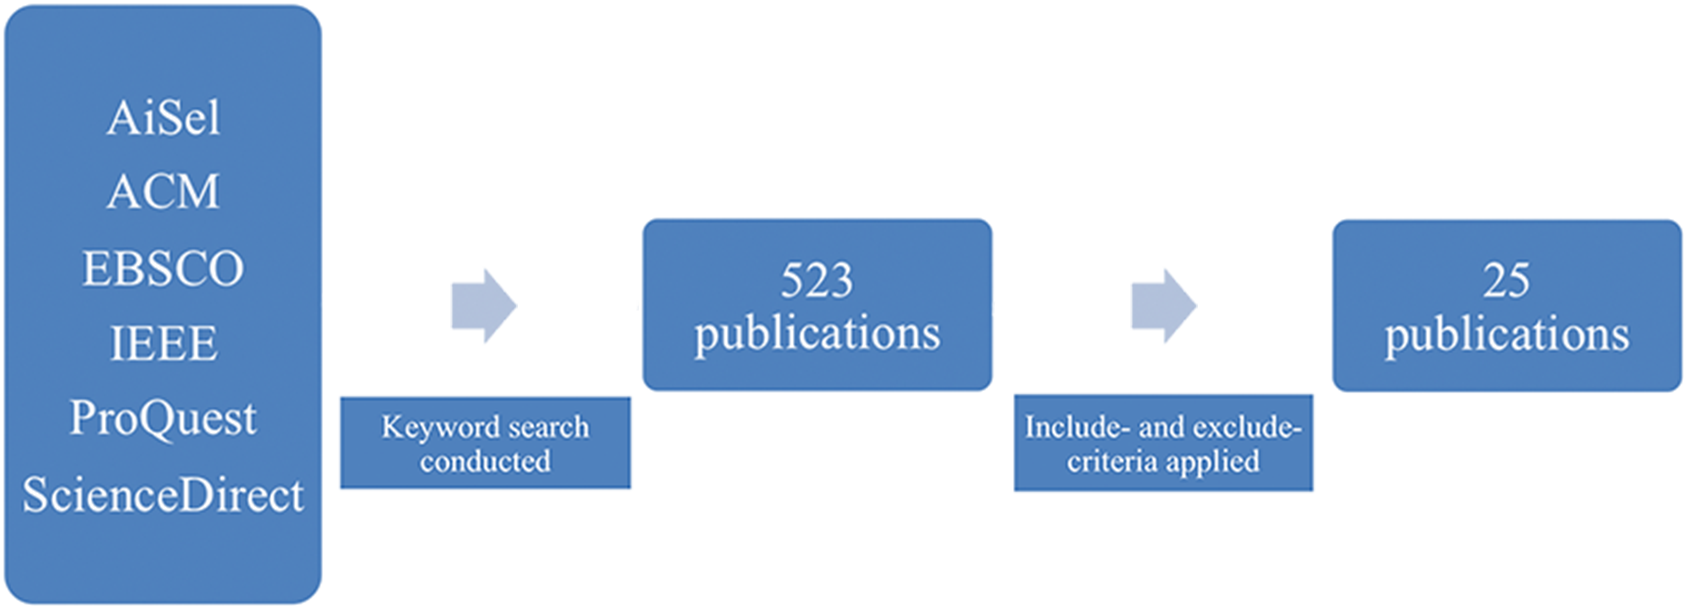
\includegraphics[width=\linewidth]{figures/research_approach_part_1.png}
    \caption[Research Approach: Data Gathering]{Research Approach: Data Gathering}
    \label{fig:ResearchApproachGathering}
\end{figure}

\begin{table}[ptbh]
    \center
    \begin{tabular}{p{16.75em} | p{16.75em}}
        \textbf{Include Criteria} & \textbf{Exclude Criteria} \\
        \hline
        Empirical works & Theoretical works, grey literature, dissertations \\
        A teaching problem is solved with the help of \AR or a teaching concept is improved by \AR & Untried or untested technologies, concepts without empirical evidence \\
        Lists positive effects of \AR applications in comparison to conventional learning tools & No control-group or control-scenario provided, no comparison to conventional learning tools \\
        Human learning & Machine learning \\
        English language & Other language \\
        Peer-reviewed & Not peer-reviewed \\
        Students without disabilities or special requirements & Students with disabilities or special requirements \\
    \end{tabular}
    \caption[Include- and Exclude-Criteria]{Include- and Exclude-Criteria}
    \label{tab:IncludeExcludeCriteria}
\end{table}

\begin{figure}[ptbh]
    \centering
    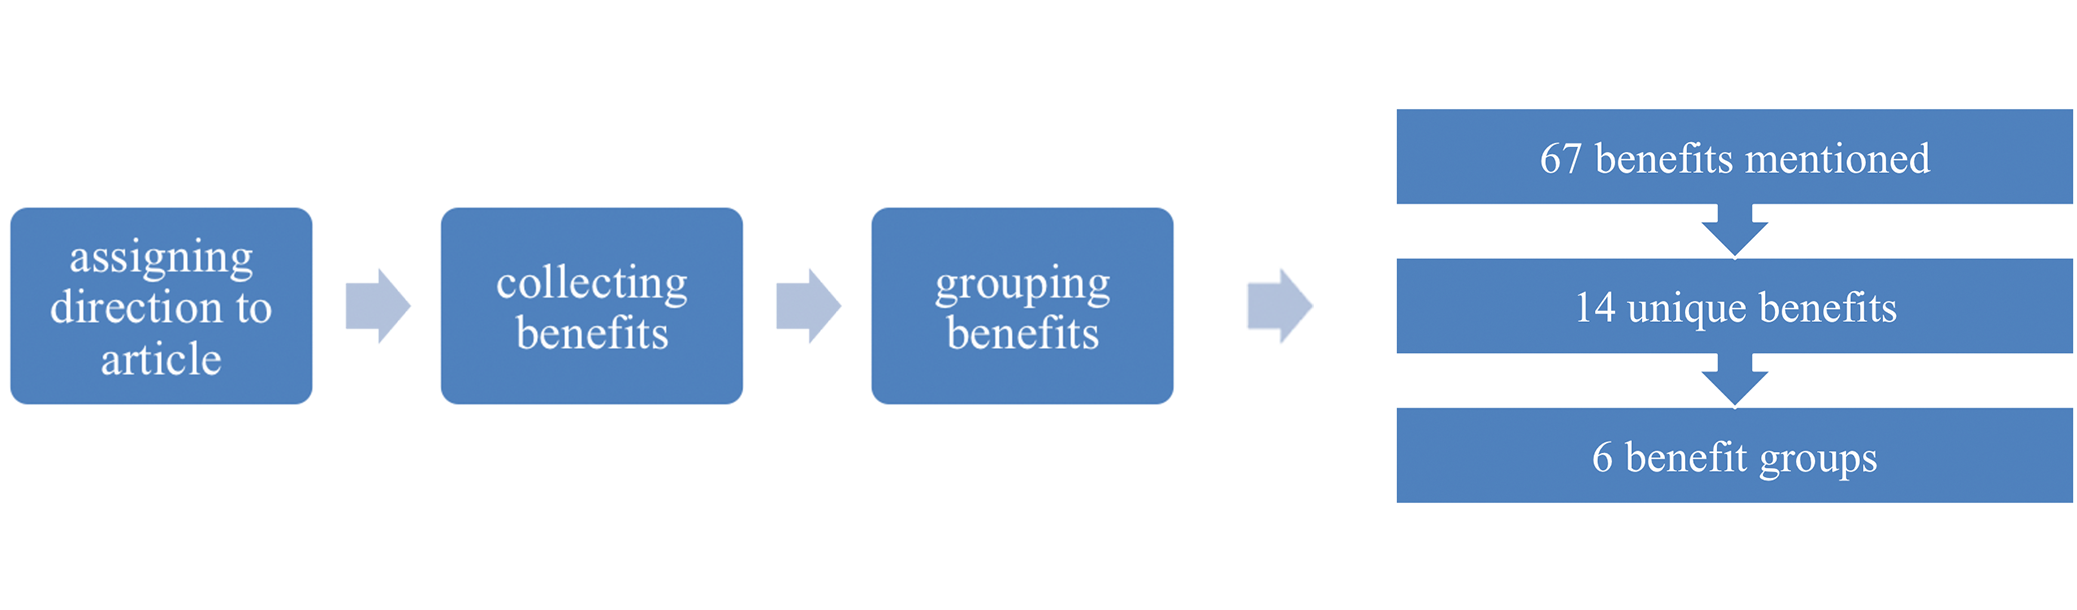
\includegraphics[width=\linewidth]{figures/research_approach_part_2.png}
    \caption[Research Approach: Data Analysis]{Research Approach: Data Analysis}
    \label{fig:ResearchApproachAnalysis}
\end{figure}

\subsection{Data Analysis}
\label{subsec:DataAnalysis}
During data analysis we clustered all found benefits into major groups and matched all found benefits to the directions of the articles in which they were mentioned. We will go into details regarding the benefits found and the clustering of them in chapter \ref{subsec:Benefits} and the mapping process will be highlighted in chapter \ref{subsec:Mapping}.\\
Because of our orientation towards the five directions, we assigned preliminary directions to all articles during data collection but revised our assignment in case of differences between the first and second coder. To measure our precision regarding the coding of the articles into directions, we utilised the inter-coder reliability score, proposed by \cite{Miles.1994}.\autocite[cf.][46]{Miles.1994} This score is calculated by dividing the number of agreements by the total number of agreements and disagreements. Our inter-coder reliability score is 0.64. We will interpret and discuss this score in chapter \ref{sec:Discussion}. \\
During assignment of directions we also collected all mentioned benefits and generalised similar benefits into a single one. Afterwards, those benefits were grouped into broader topic-related benefits. The process we applied is based on the process proposed by \cite{Jankowicz.2004}.\autocite[cf.][149]{Jankowicz.2004} The process proposed by \cite{Jankowicz.2004} helps by formalising the process of clustering.\\
A total of 99 quotes were collected and 67 benefits were mentioned, containing 14 unique benefits, which were clustered into six clusters. In the next chapter, we will introduce all found benefits and their major groups.